%Author: Alexander Feng
%Problem is just your plain old manual convolution.

\qns{Manual Convolution}

\meta{Ask students if there may be something peculiar that $g$ may do if we convolve it with a given signal.}

Given two discrete time signals $f$ and $g$, recall that the convolution of $f$ and $g$ is given by 
\begin{align*}
(f * g)[n] = \sum^{\infty}_{k = -\infty} f[k]g[n-k]
\end{align*}

Convolve the following two finite discrete time signals and draw the corresponding plot:

Graph of $f$: 

\begin{center}
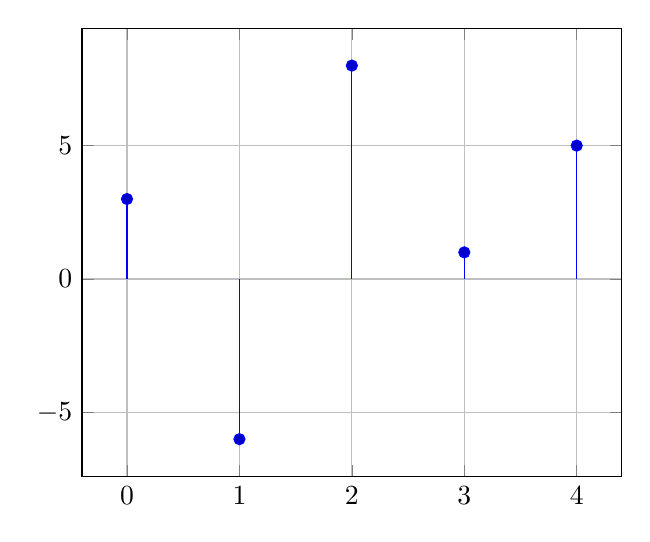
\begin{tikzpicture}
    \begin{axis}[
        xmajorgrids=true, ymajorgrids=true]
    \addplot+[ycomb] plot coordinates
        {(0,3) (1,-6) (2,8) (3,1) (4,5)};
    \end{axis}
\end{tikzpicture}
\end{center}

Graph of $g$:

\begin{center}
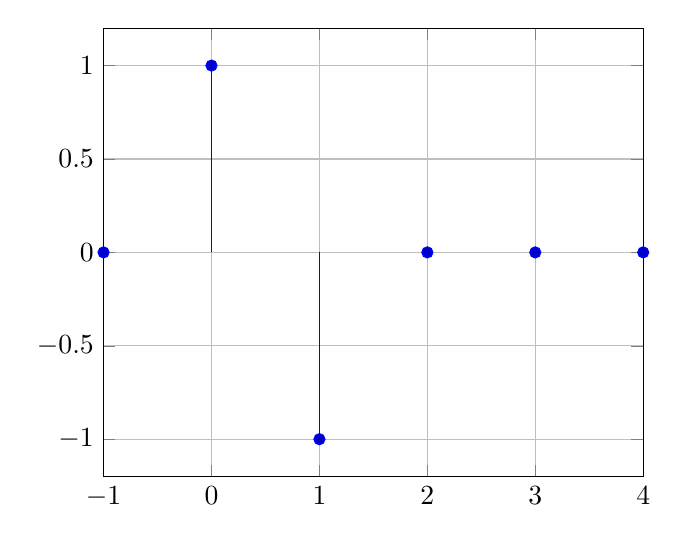
\begin{tikzpicture}
    \begin{axis}[xmin = -1, xmax = 4, 
        xmajorgrids=true, ymajorgrids=true]
    \addplot+[ycomb] plot coordinates
        {(-1, 0) (0, 1) (1, -1) (2, 0) (3, 0) (4, 0)};
    \end{axis}
\end{tikzpicture}
\end{center}

\sol{
    We get the following: 
    \begin{center}
        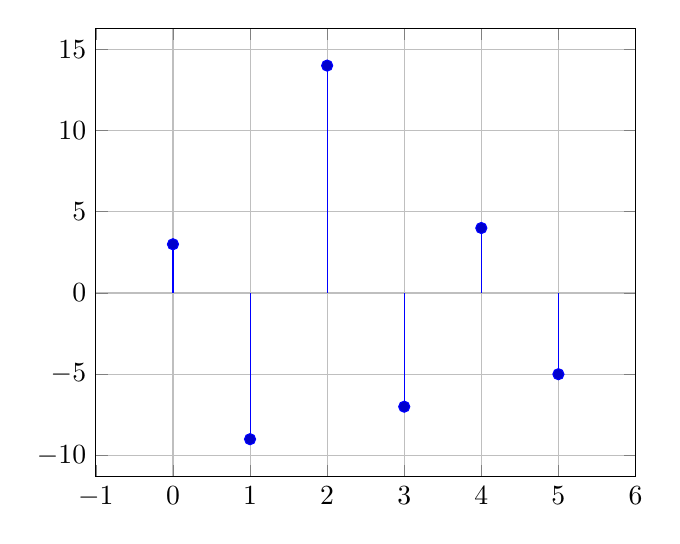
\begin{tikzpicture}
            \begin{axis}[xmin = -1, xmax = 6, 
                xmajorgrids=true, ymajorgrids=true]
            \addplot+[ycomb] plot coordinates
                {(0, 3) (1, -9) (2, 14) (3, -7) (4, 4) (5, -5)};
            \end{axis}
        \end{tikzpicture}
        \end{center}

    As it turns out, convolving a signal with $g$ can be used in edge detection as the convolved signal will have large outputs where there are large differences in concurrent values.
    If we were to use an image with RGB values, using a similar signal but in 2D, we'd be able to see where there're large fluctuations in RGB values (ex. person and background).
}